\chapter{Results \& Discussion}
\label{Chapter4}
\lhead{Chapter 4. \emph{Results \& Discussion}}

\section{Convergency Tests}
\subsection{Cut-off Energy}
\subsection{K-Points Sampling}
\section{Density of States (DOS)}



Hello




\begin{figure}[h]
    \centering
    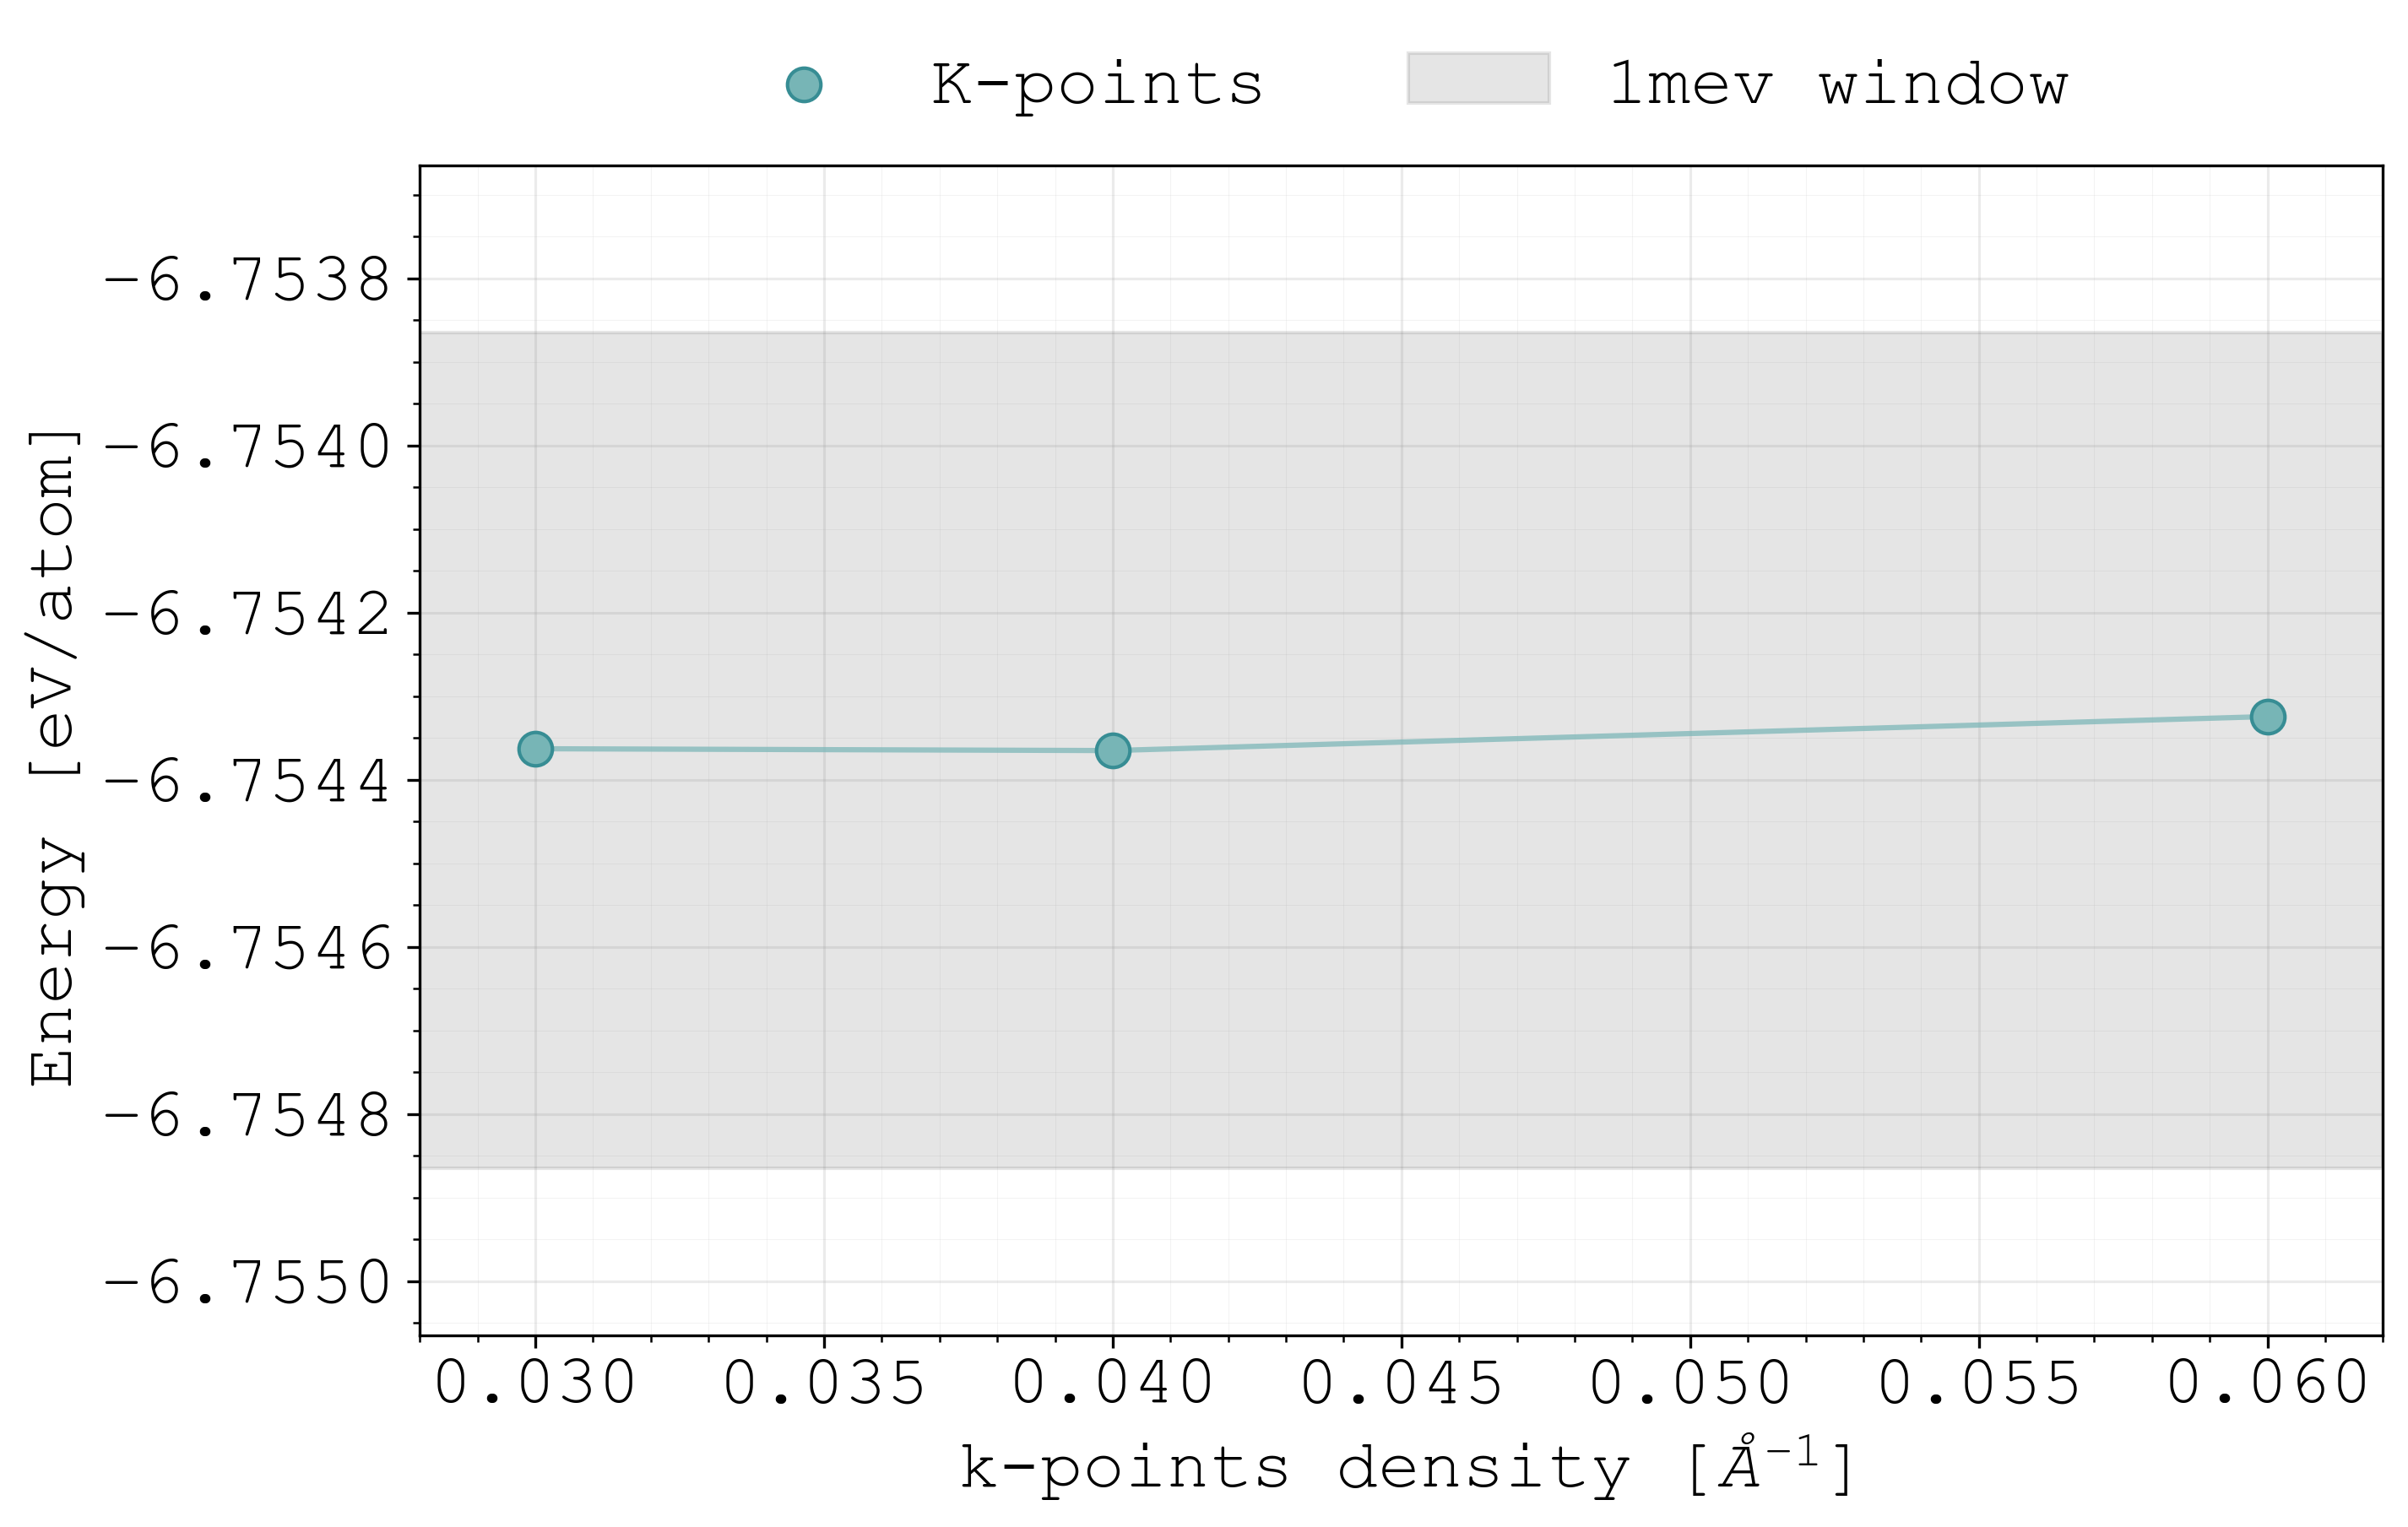
\includegraphics[width=0.8\textwidth]{dftb-kpoints.png}
    \caption{k-point convergence test performed in DFTB+ using the GFN1-xTB method for $0.03 \leq \Delta k \leq 0.06$. The 
    $\Delta E = 1$meV/atom convergence criteria is achieved at $\Delta k = 0.06 \,\text{\AA}^{-1}$ corresponding to a $1\times 1\times 1$ k-point grid.
    }
    \label{dftb-kpoints}
\end{figure}

\begin{figure}[h]
    \centering
    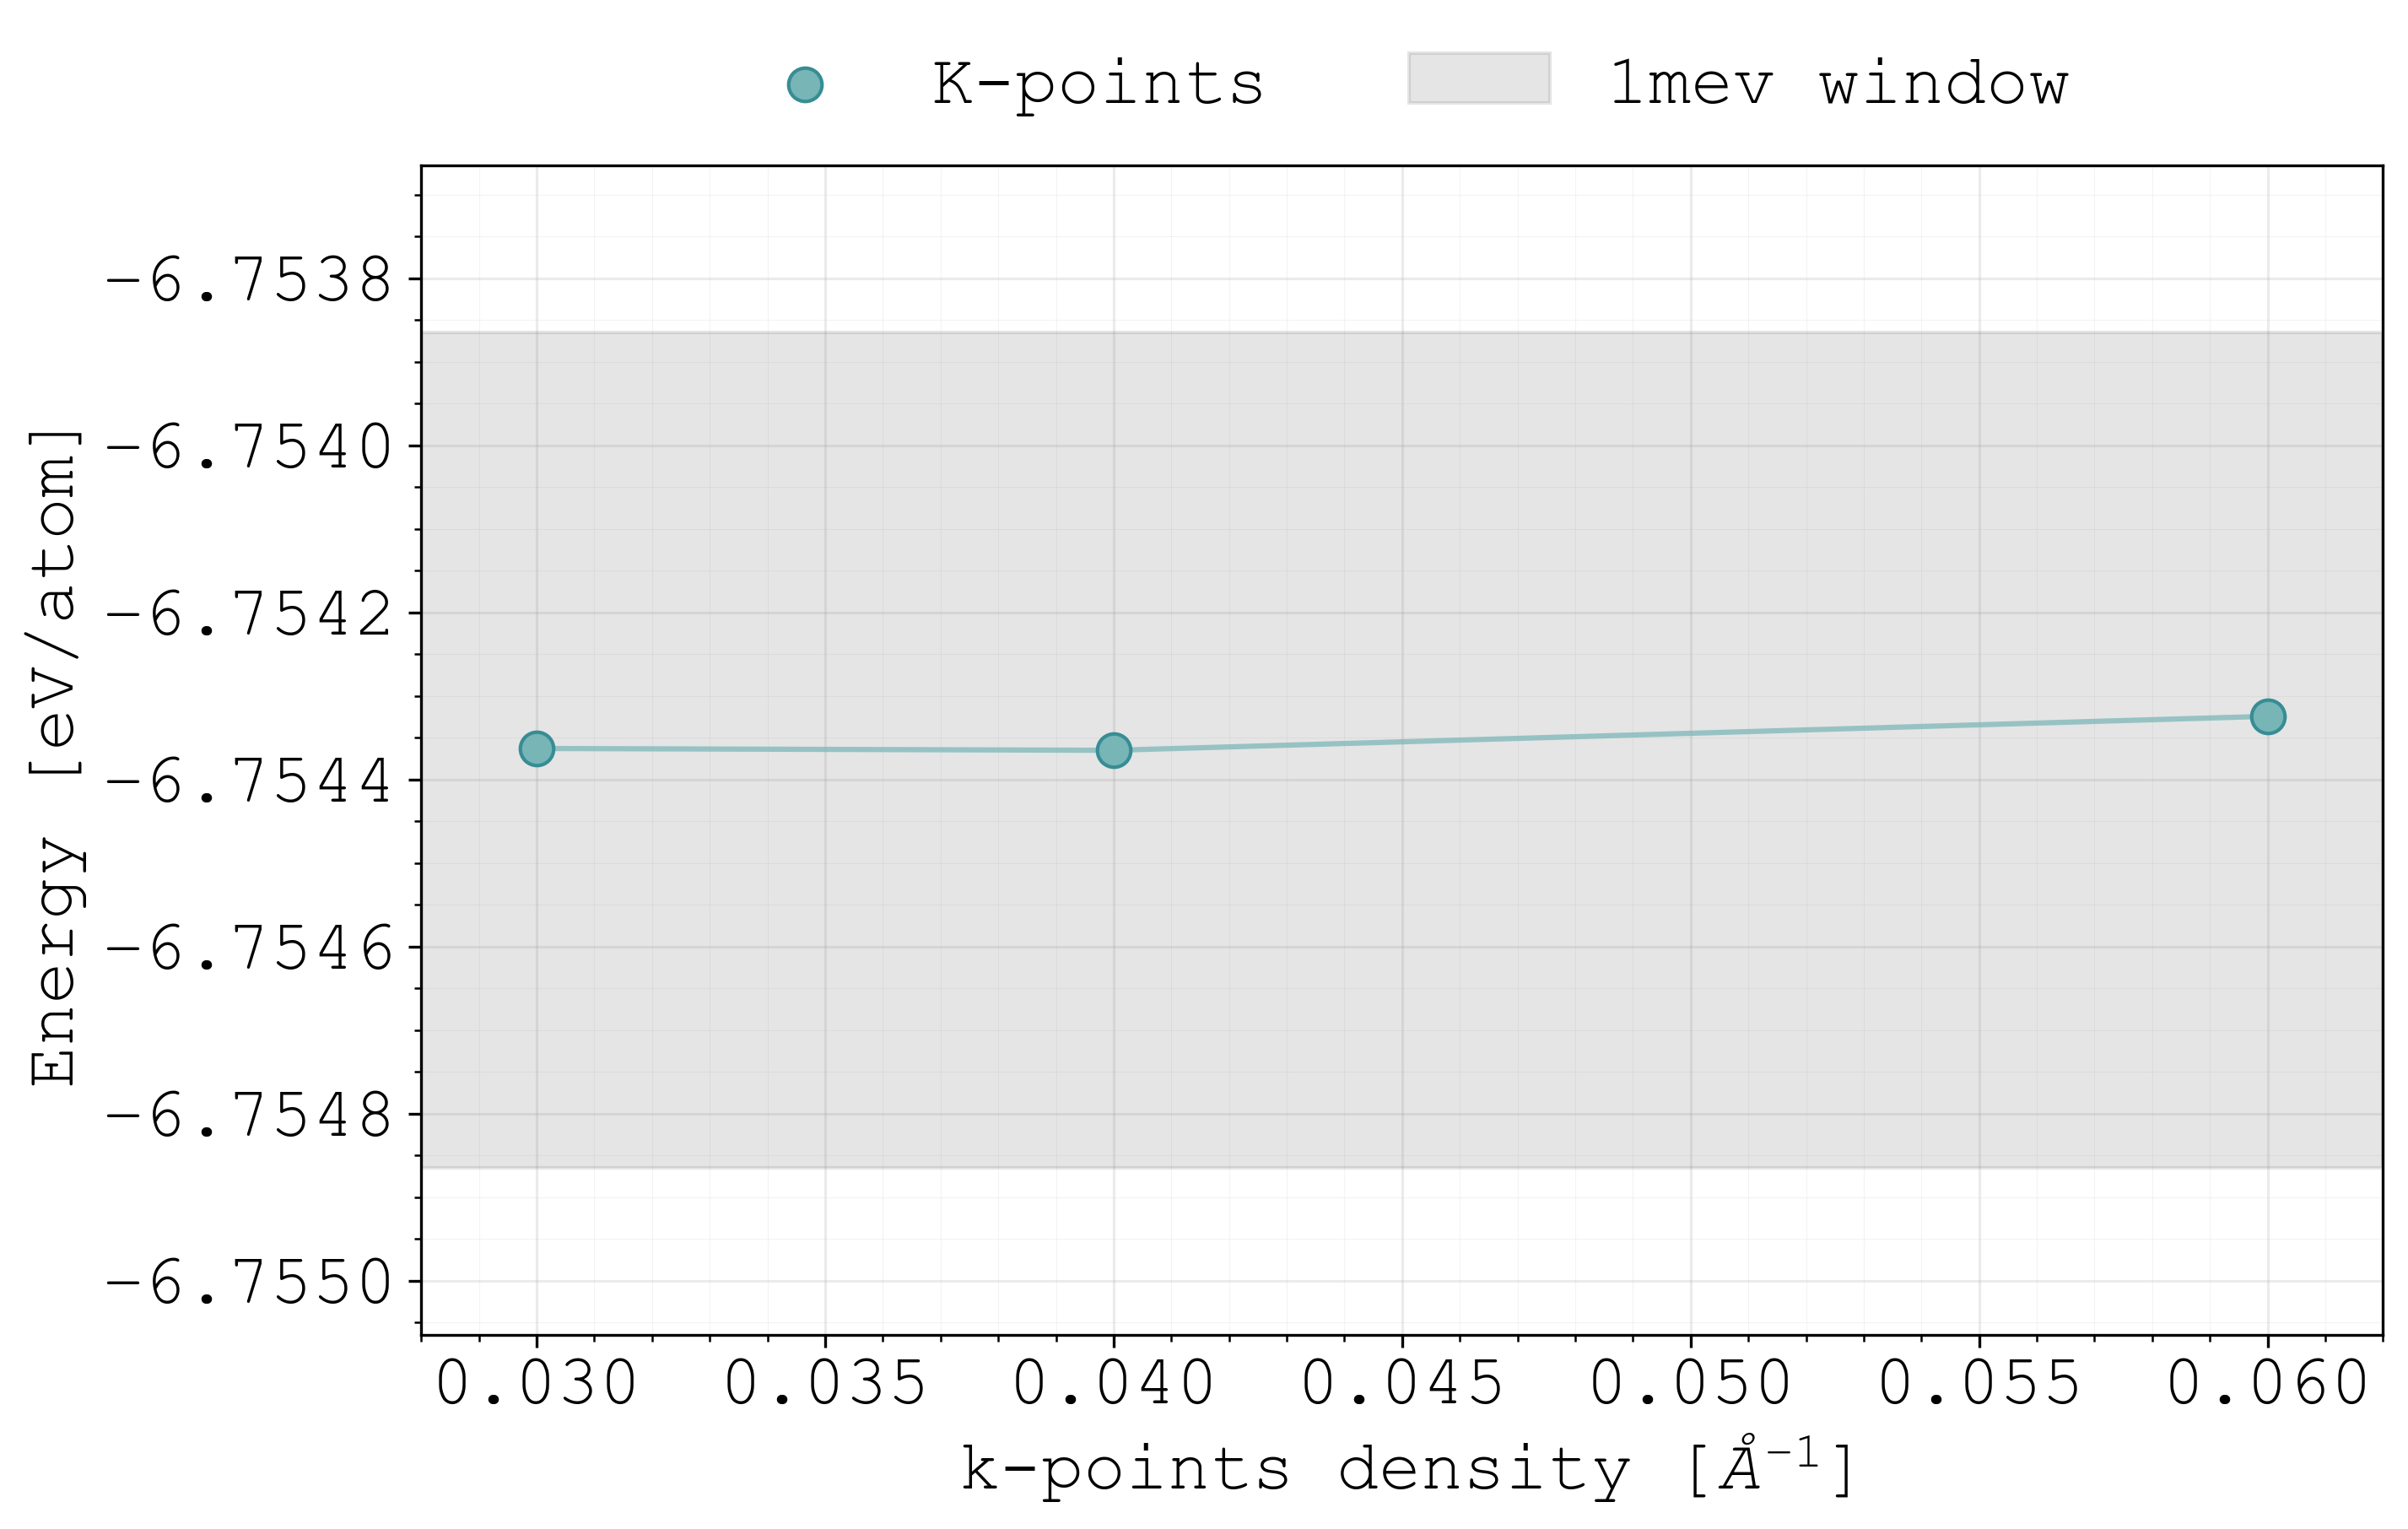
\includegraphics[width=0.8\textwidth]{kpoints-vasp.png}
    \caption{k-point convergence test performed in VASP using the PBEsol functional for $0.03 \leq \Delta k \leq 0.06$. The $\Delta E = 1$meV/atom convergence criteria is achieved at $\Delta k = 0.06 \,\text{\AA}^{-1}$ corresponding to a $1\times 1\times 1$ k-point grid, in agreement with the DFTB+ results.
    }
    \label{kpoints-vasp}
\end{figure}

\begin{figure}[h]
    \centering
    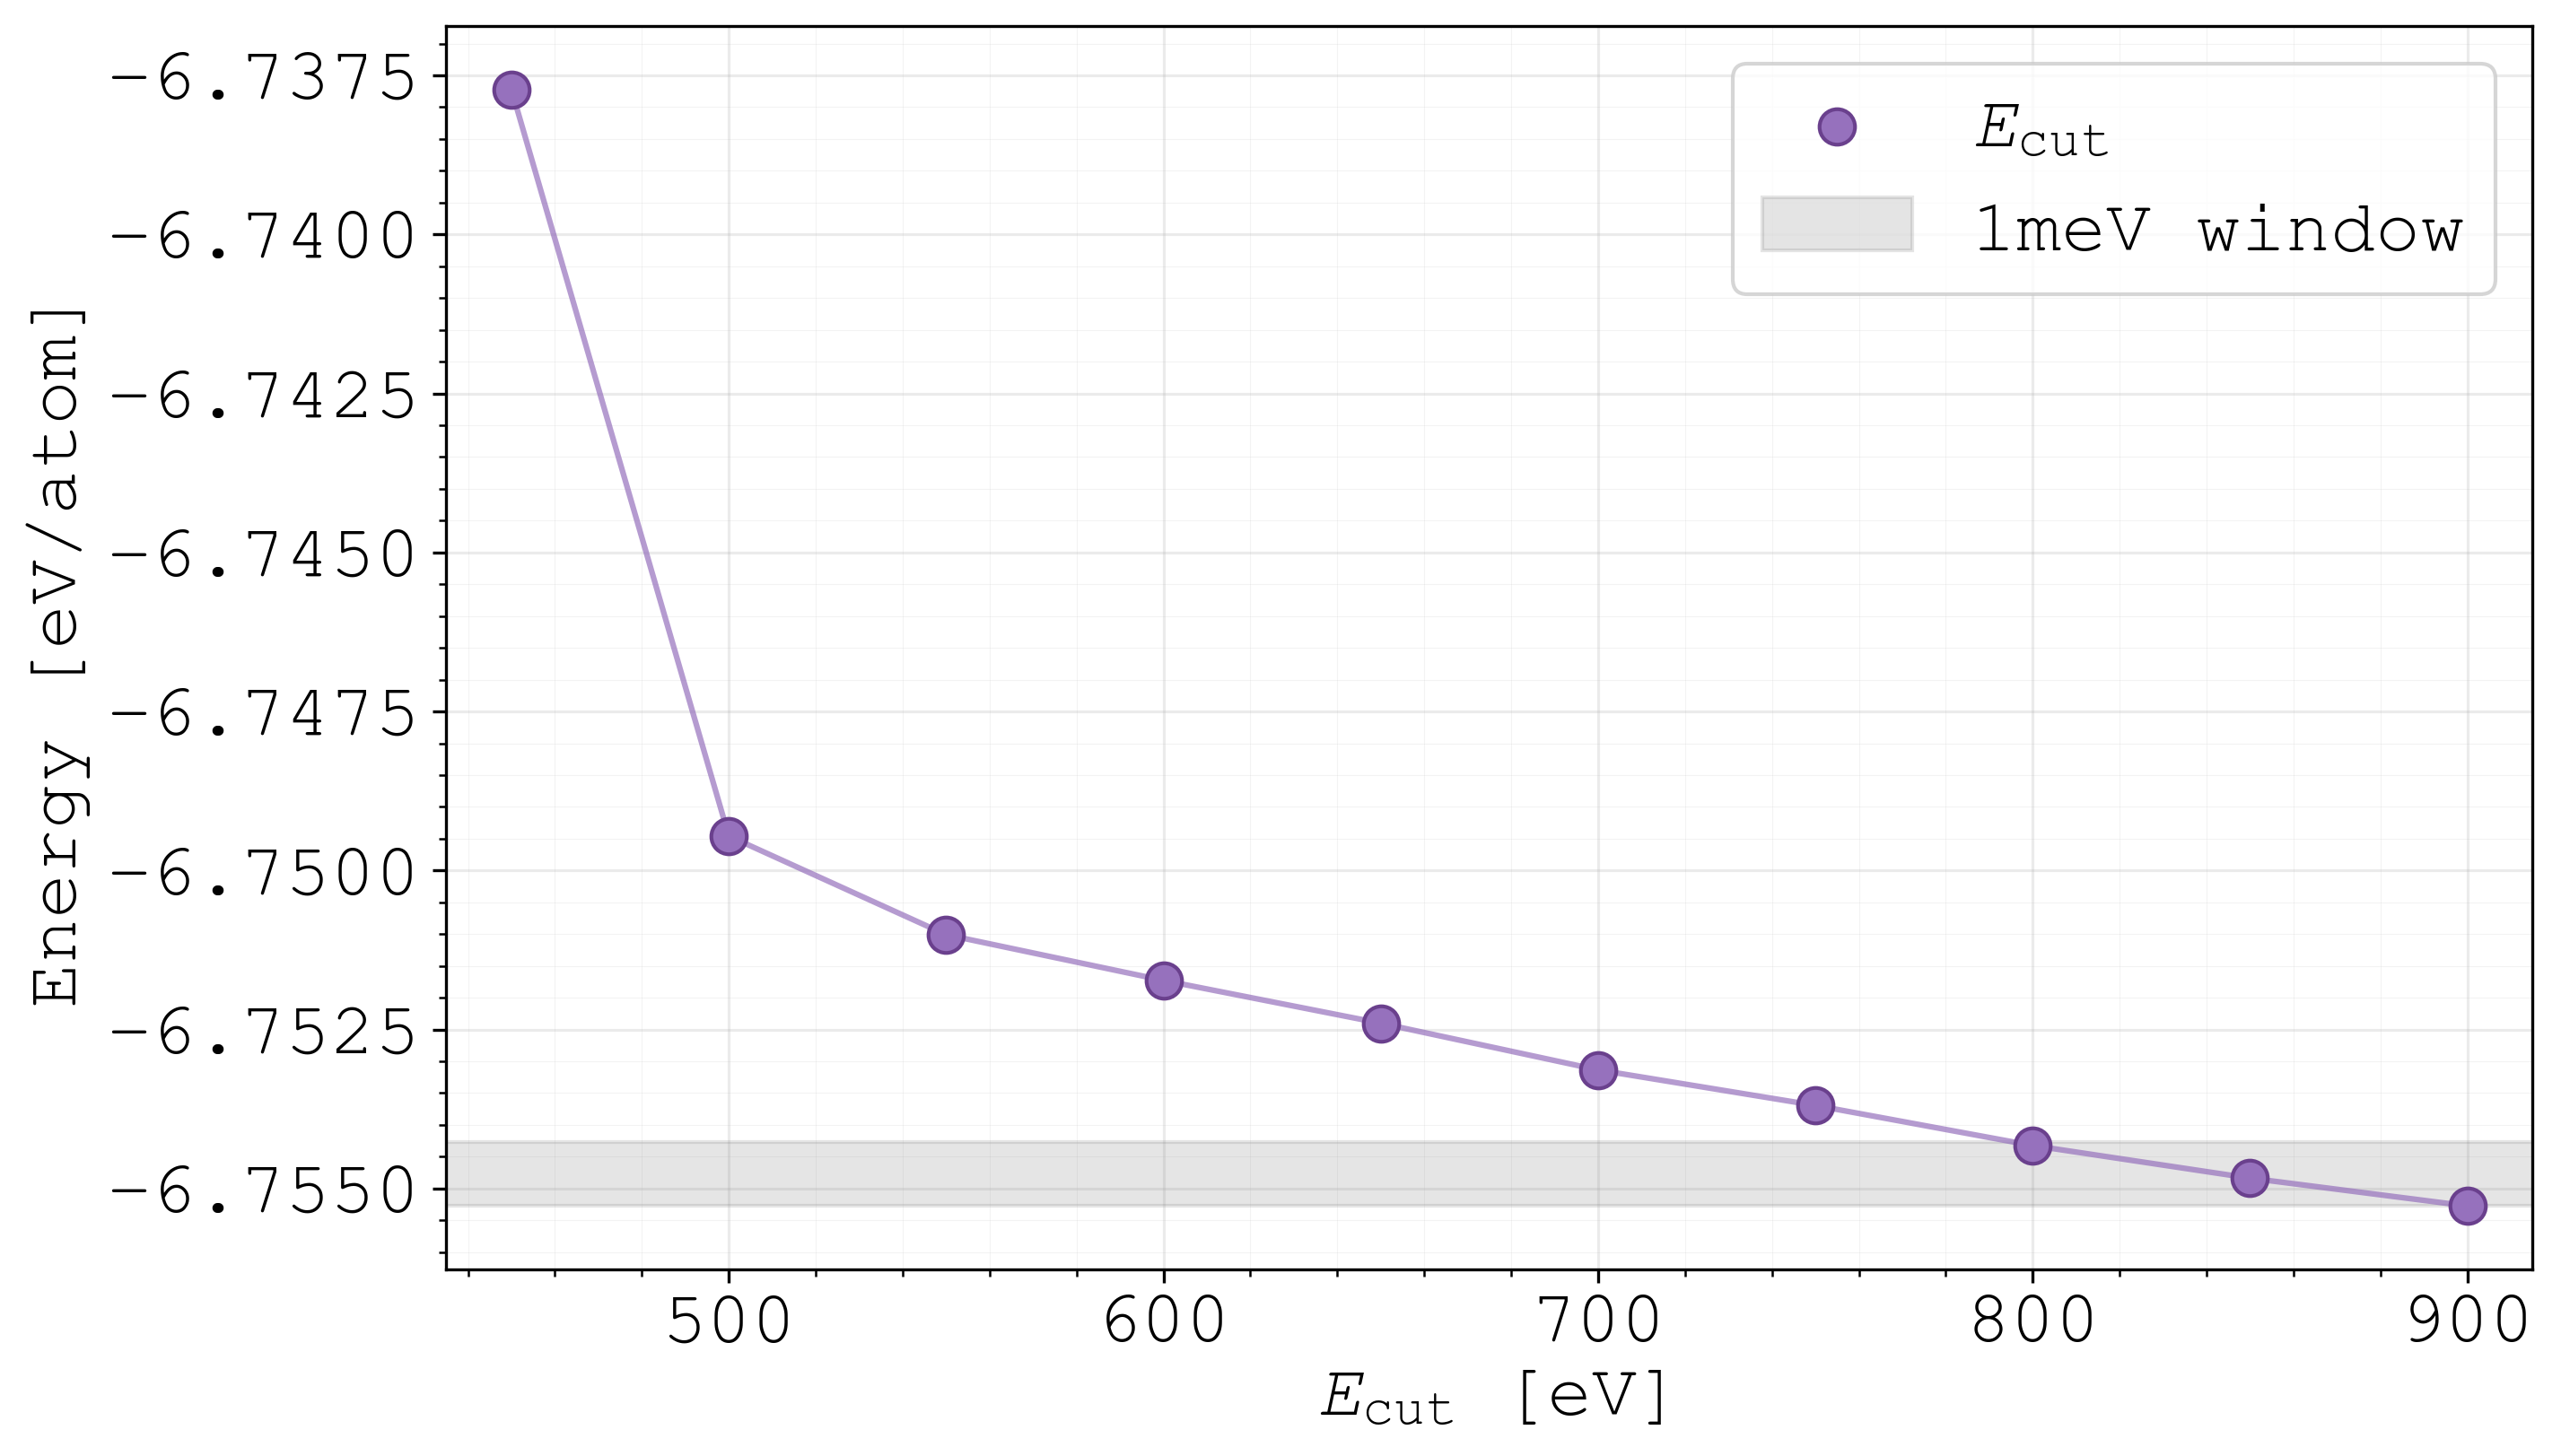
\includegraphics[width=0.8\textwidth]{cutoff-vasp.png}
    \caption{
    Cut-off energy convergence test performed in VASP employing the PBEsol functional for $300 \leq E_{\text{cut}} \leq 900$ eV. The $\Delta E = 1$meV/atom convergence criteria is achieved at $E_{\text {cut}} = 800$ eV}
    \label{cutoff-energy}
\end{figure}

\begin{figure}[h]
    \centering
    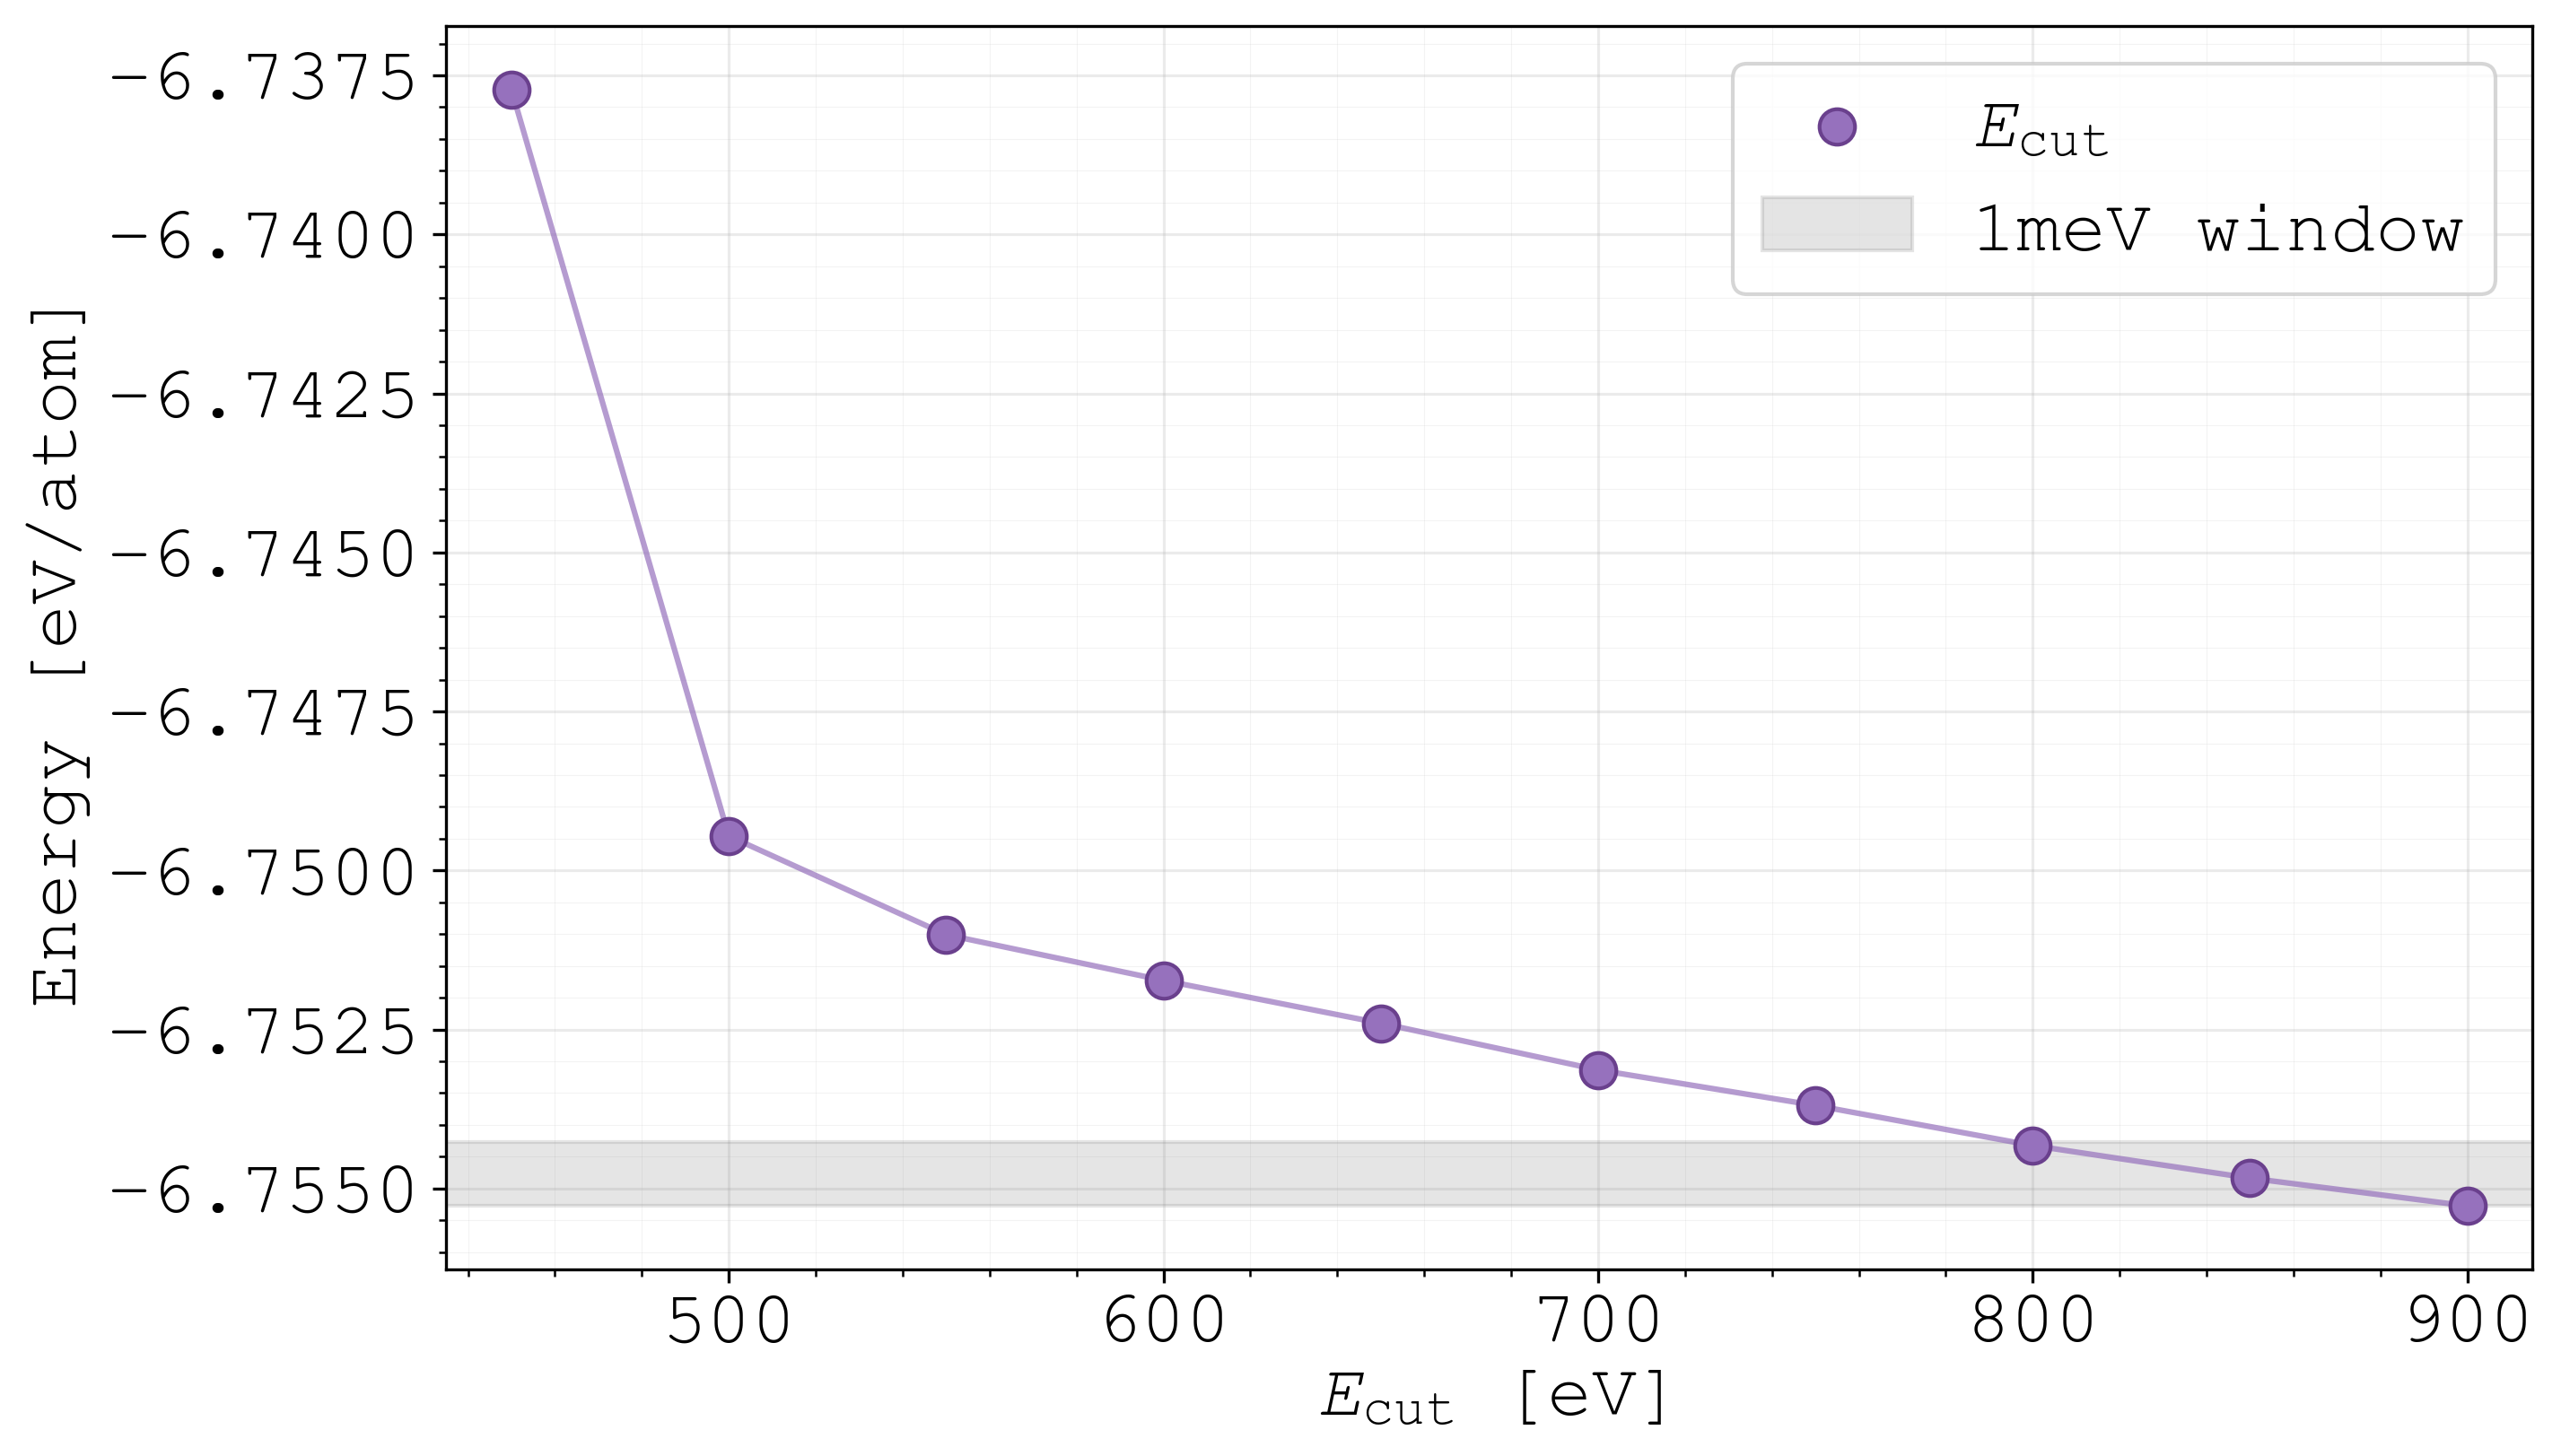
\includegraphics[width=0.8\textwidth]{cutoff-vasp.png}
    \caption{
    Cut-off energy convergence test performed in VASP employing the PBEsol functional for $300 \leq E_{\text{cut}} \leq 900$ eV. The $\Delta E = 1$meV/atom convergence criteria is achieved at $E_{\text {cut}} = 800$ eV}
    \label{cutoff-energy}
\end{figure}



\begin{figure}[h]
    \centering
    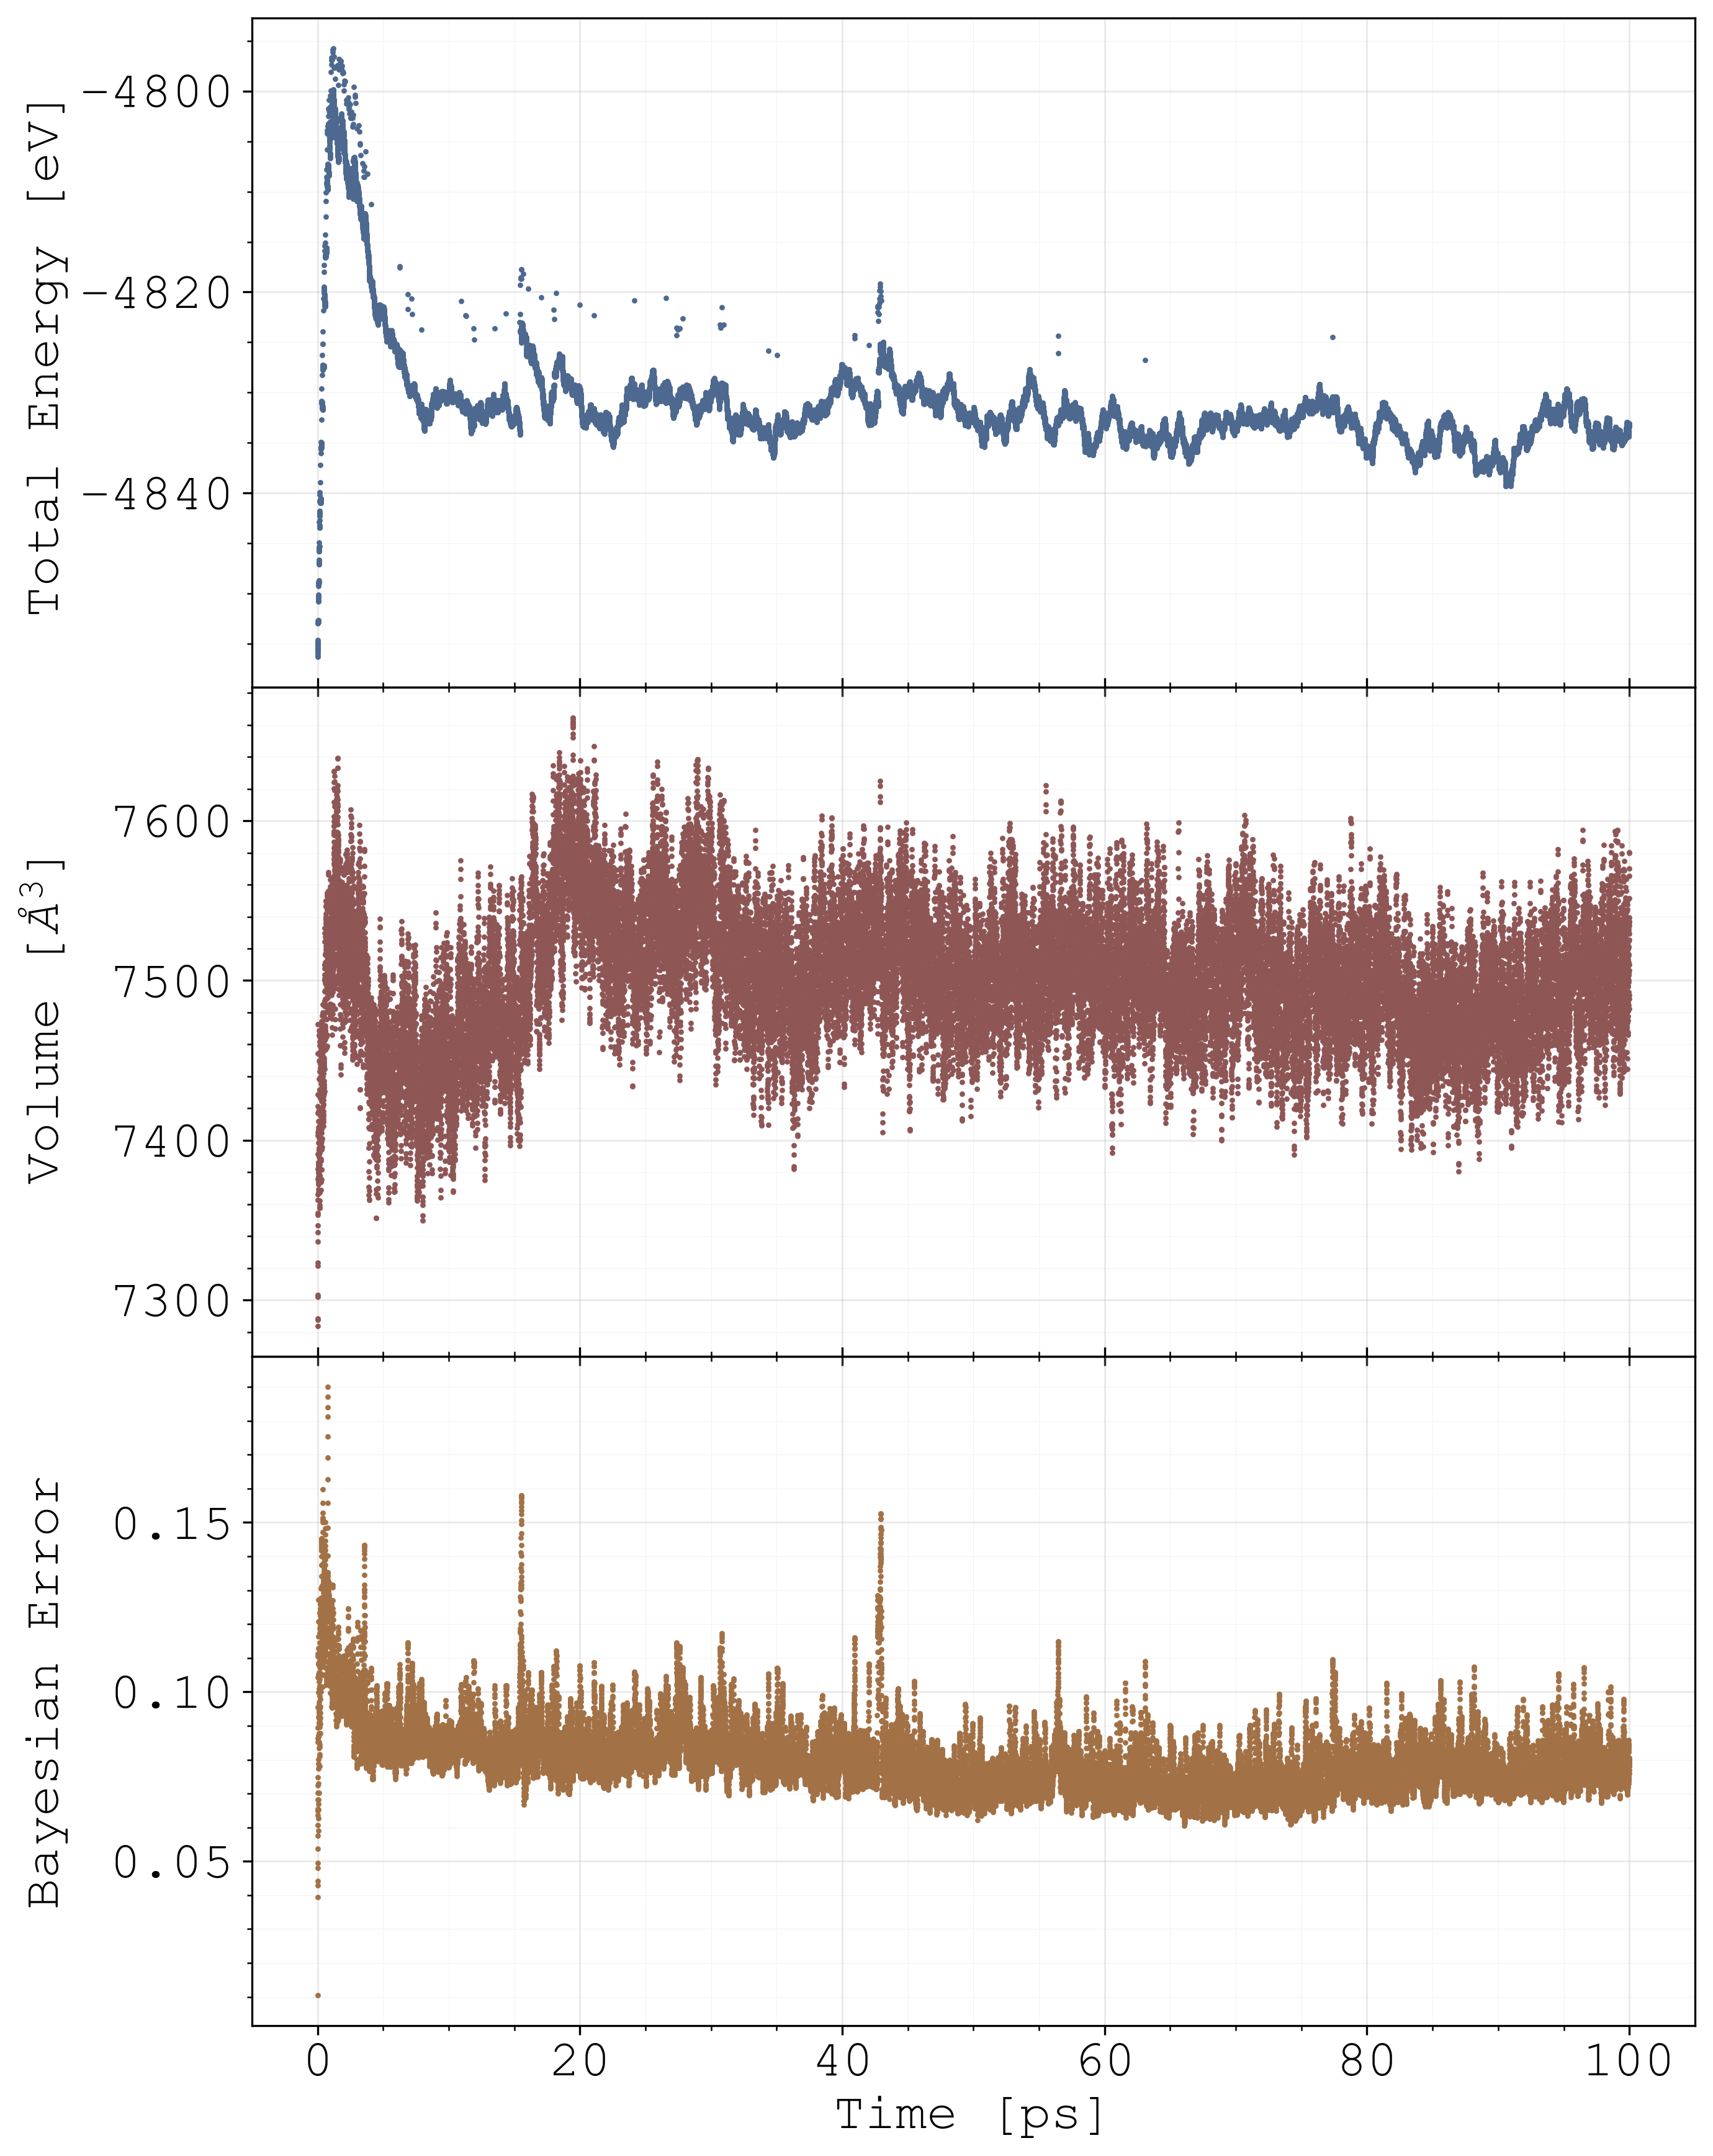
\includegraphics[width=0.8\textwidth]{training-stats.png}
    \caption{
    My label
    }
    \label{training-stats}
\end{figure}

\begin{figure}[h]
    \centering
    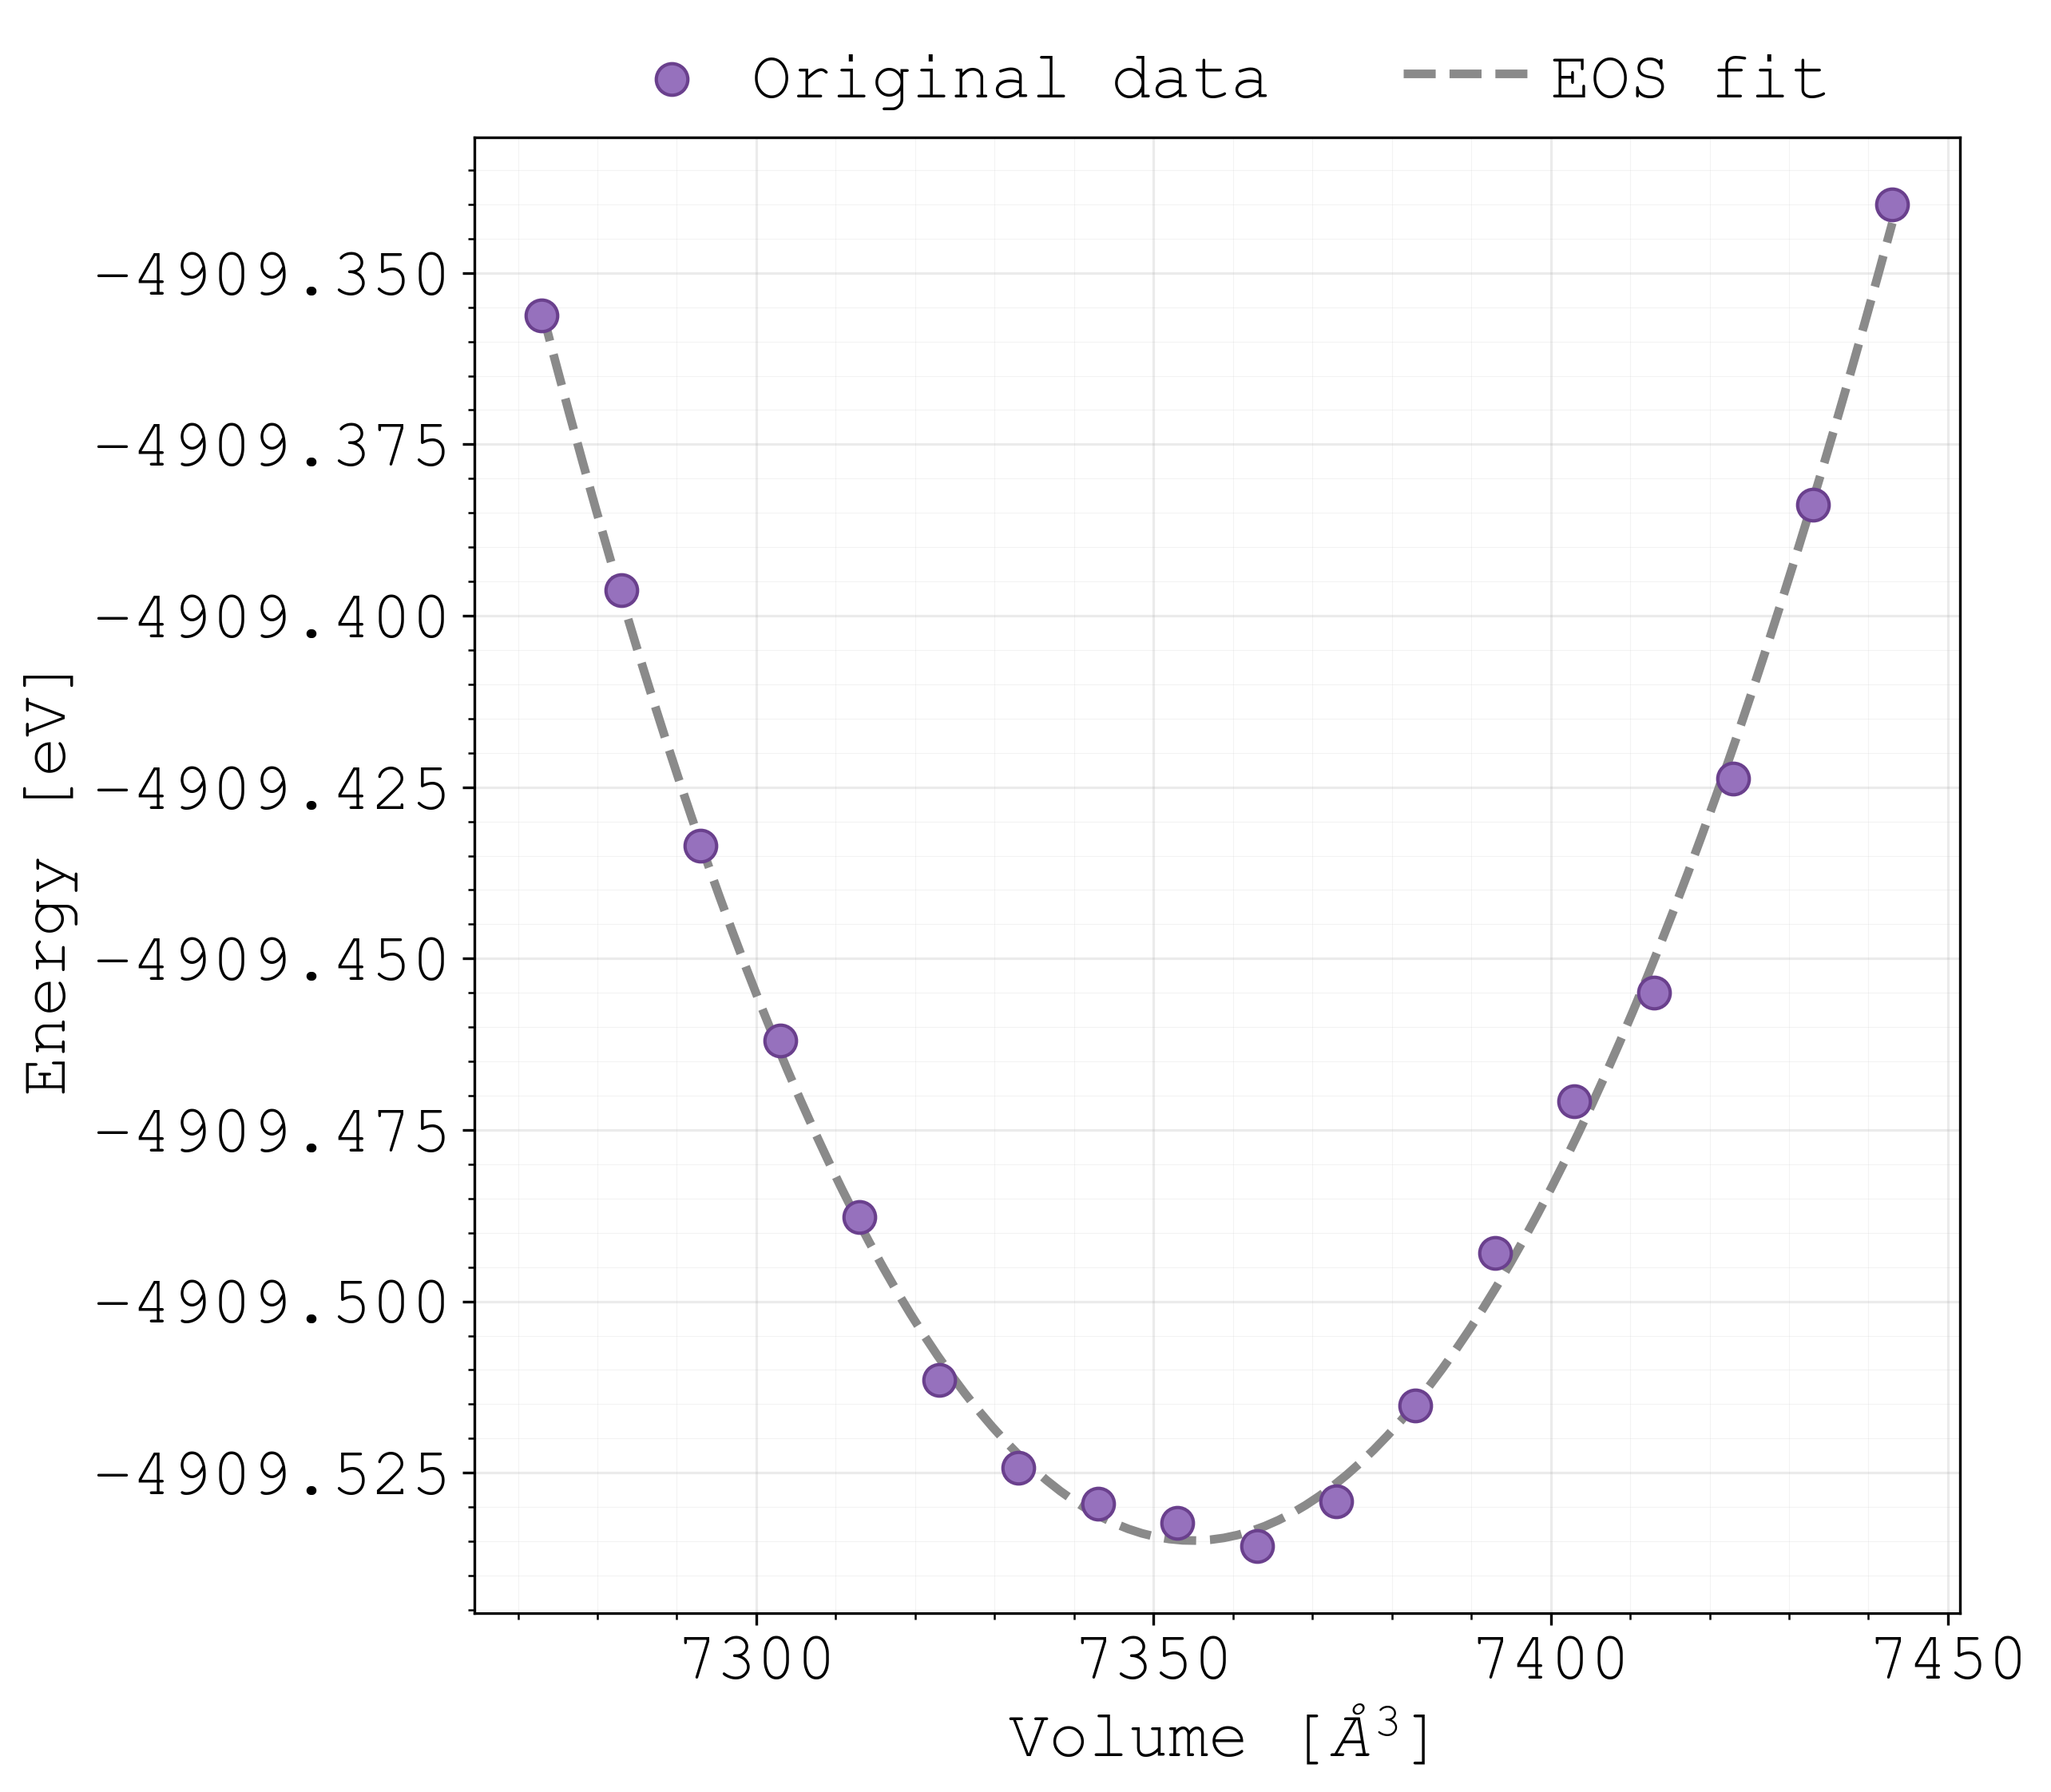
\includegraphics[width=0.7\textwidth]{EOS_SA_EDIFF_02.png}
    \caption{A schematic representation of the DFT formalism. The many-body wavefunction is replaced by a single-particle wavefunction, which is used to calculate the electron density. The electron density is then used to calculate the total energy of the system. Adapted from \supercite{giustino2014materials}.}
    \label{fig:dft}
\end{figure}